%!TEX root = ../thesis.tex
%*******************************************************************************
%*********************************** First Chapter *****************************
%*******************************************************************************

\chapter{Tokamak-shape Application}  %Title of the First Chapter

\ifpdf
    \graphicspath{{Chapter9/Figs/Raster/}{Chapter9/Figs/PDF/}{Chapter9/Figs/}}
\else
    \graphicspath{{Chapter9/Figs/Vector/}{Chapter9/Figs/}}
\fi

\label{chapter 9}


%************************************************************************** 

In the last chapter, we validate the boundary conditions and solvers with cylindrical equilibrium test. In this chapter, we apply this test in a container that more closely resembles a tokamak vessel. We build up a chamber similar to tokamak vessel in Ferraro \textit{et al.} \cite{ferraro2016multi}. We use tungsten as the vessel wall material. Hence, the resistivity is $5.6 \times 10^{-8} \, \Omega \cdot \text{m}$. The whole simulation is conducted under numerical domain of $[0.2,3.3]\times[-2.5,2.5]$ with $310\times500$ resolution. We extend the simulation to $t_{stop}=0.8$. 

The result is demonstrated in Figure \ref{fig:tokamak_application}. This simulation in the tokamak-shaped vessel provide valuable insights into the behavior of plasma under conditions that more closely resemble practical applications. As depicted in the figures, the result demonstrate the procedure core high density plasma hitting the wall and splitting out. The interaction behavior of the fast magnetoacoustic wave is particularly interesting after they are generated during the hitting and spread out, they collide again in the lower part of the vessel.


\begin{figure}[htbp]
	\centering
	
	\vspace{-5mm}
	% Row 1
	\hspace{-6mm}
	\begin{subfigure}{0.26\textwidth}
		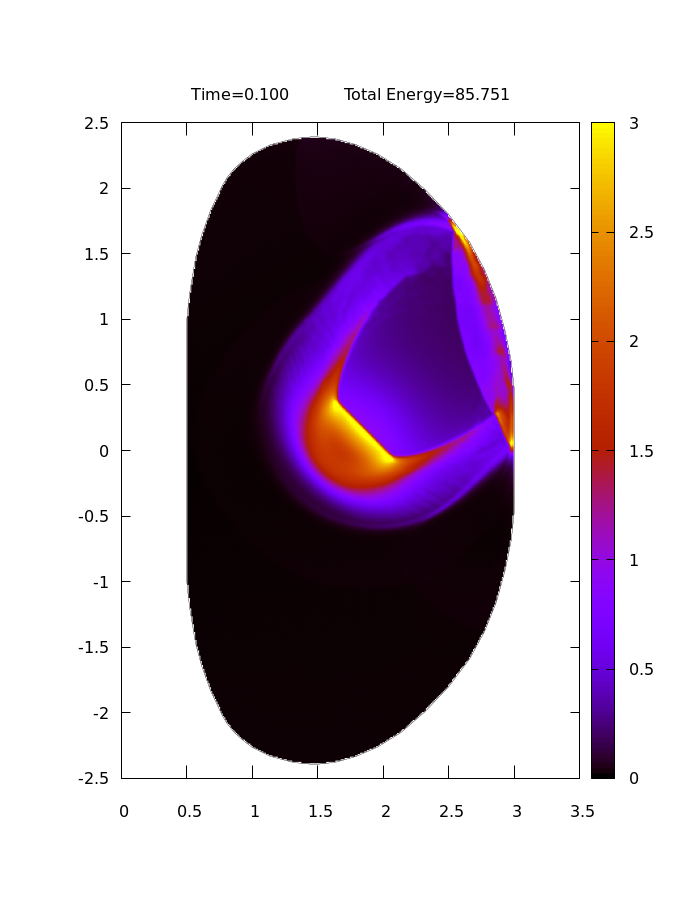
\includegraphics[width=\linewidth]{tokamak_Density_050.png}
	\end{subfigure}
	\hspace{-4mm} % Negative horizontal space
	\begin{subfigure}{0.26\textwidth}
		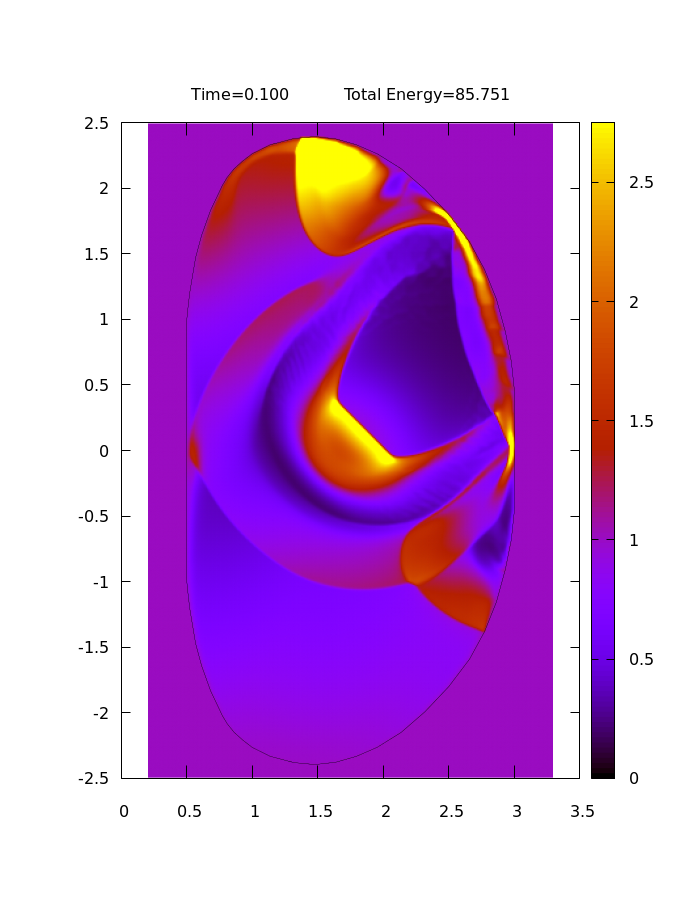
\includegraphics[width=\linewidth]{tokamak_Bz_050.png}
	\end{subfigure}
	\hspace{2mm} % Negative horizontal space
	\begin{subfigure}{0.26\textwidth}
		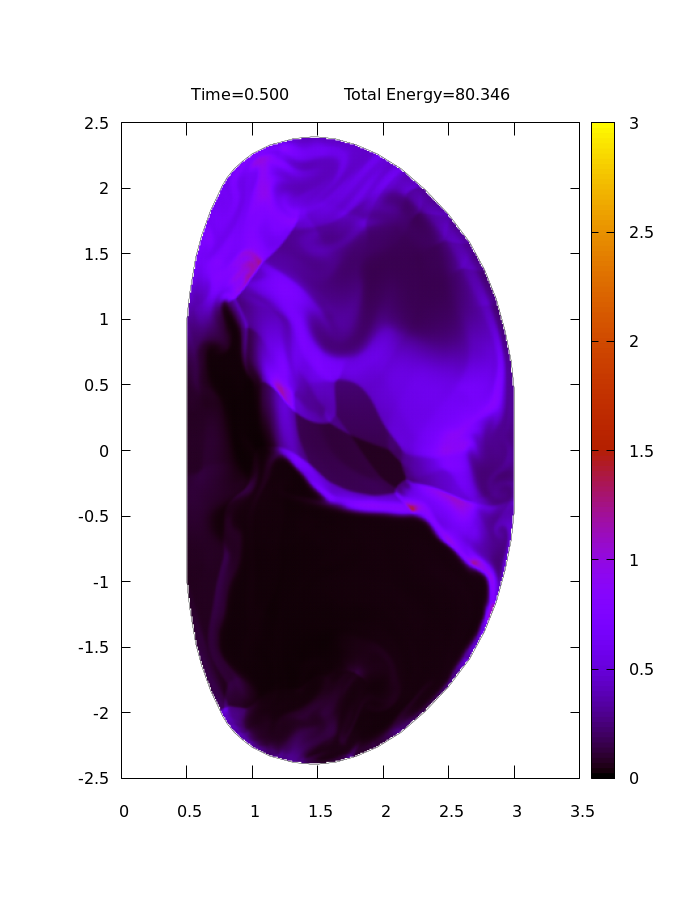
\includegraphics[width=\linewidth]{tokamak_Density_250.png}
	\end{subfigure}
	\hspace{-4mm} % Negative horizontal space
	\begin{subfigure}{0.26\textwidth}
		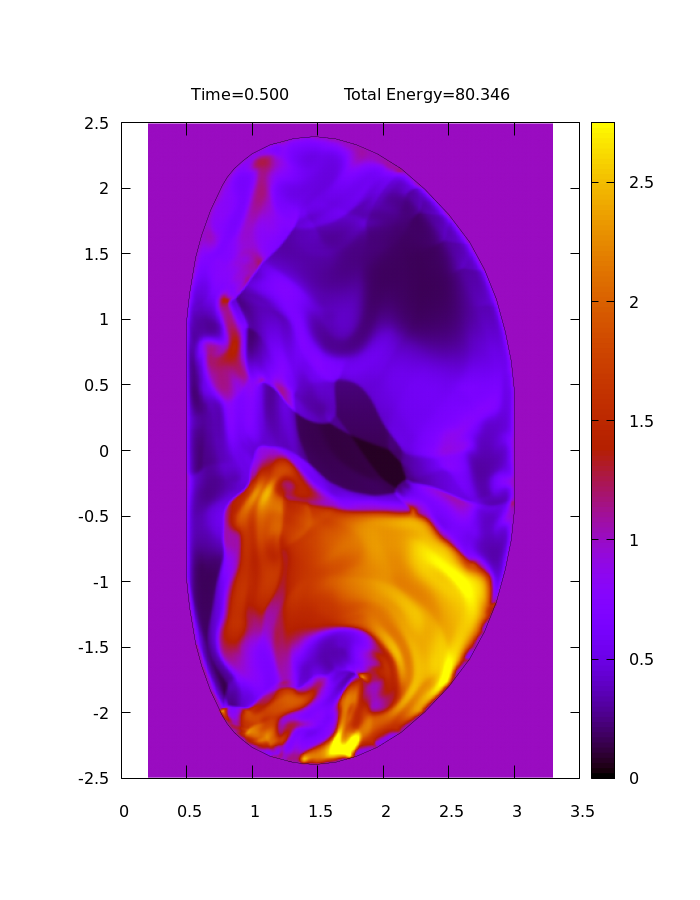
\includegraphics[width=\linewidth]{tokamak_Bz_250.png}
	\end{subfigure}
	\hspace{-6mm}
	
	\vspace{-6mm} % Negative vertical space
	
	% Row 2
	\hspace{-6mm}
	\begin{subfigure}{0.26\textwidth}
		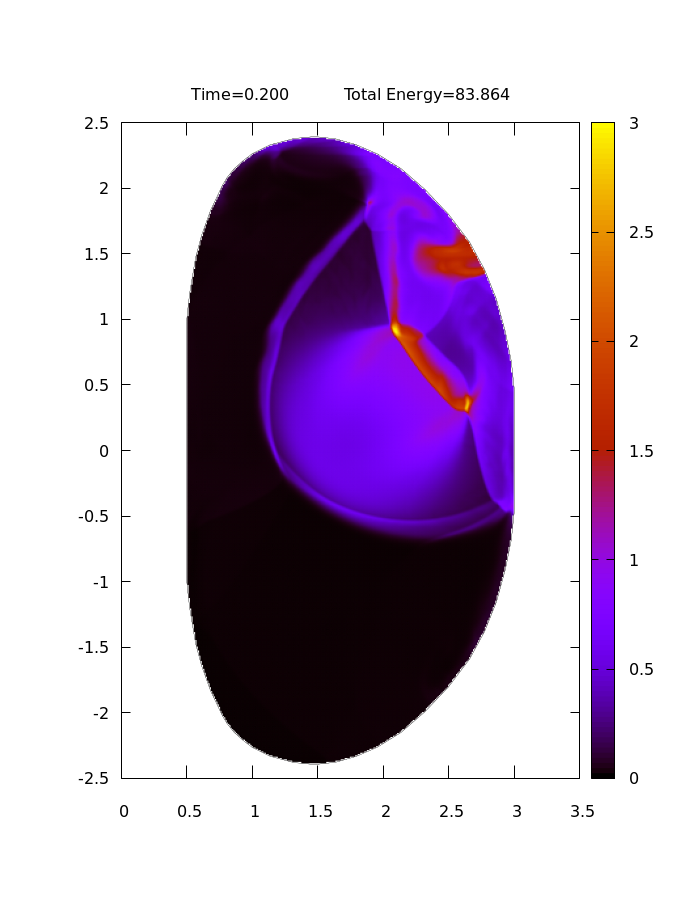
\includegraphics[width=\linewidth]{tokamak_Density_100.png}
	\end{subfigure}
	\hspace{-4mm} % Repeat negative space adjustments for each subfigure
	\begin{subfigure}{0.26\textwidth}
		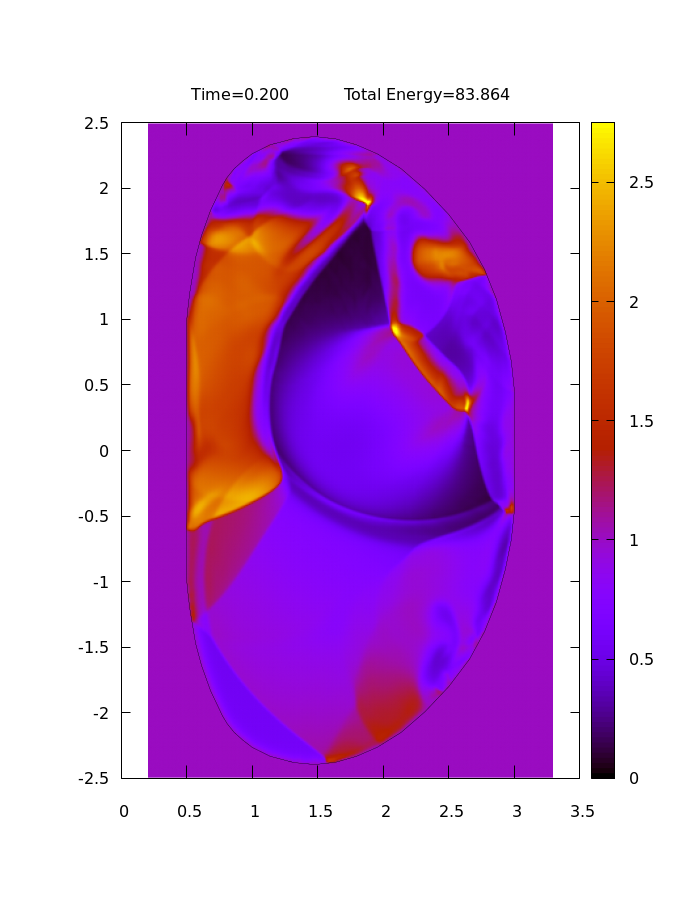
\includegraphics[width=\linewidth]{tokamak_Bz_100.png}
	\end{subfigure}
	\hspace{2mm} % Repeat negative space adjustments for each subfigure
	\begin{subfigure}{0.26\textwidth}
		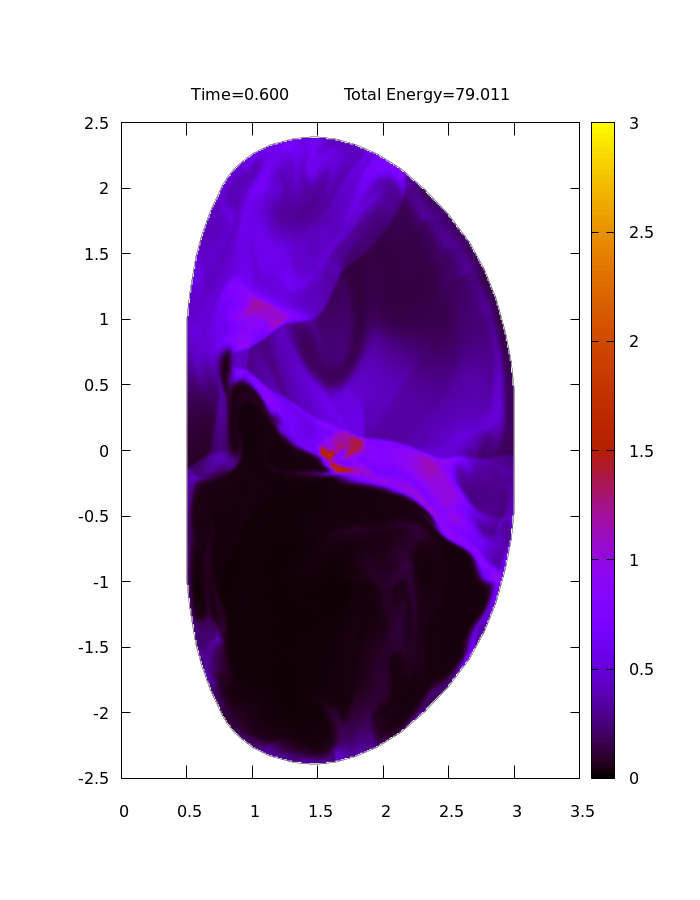
\includegraphics[width=\linewidth]{tokamak_Density_300.png}
	\end{subfigure}
	\hspace{-4mm} % Repeat negative space adjustments for each subfigure
	\begin{subfigure}{0.26\textwidth}
		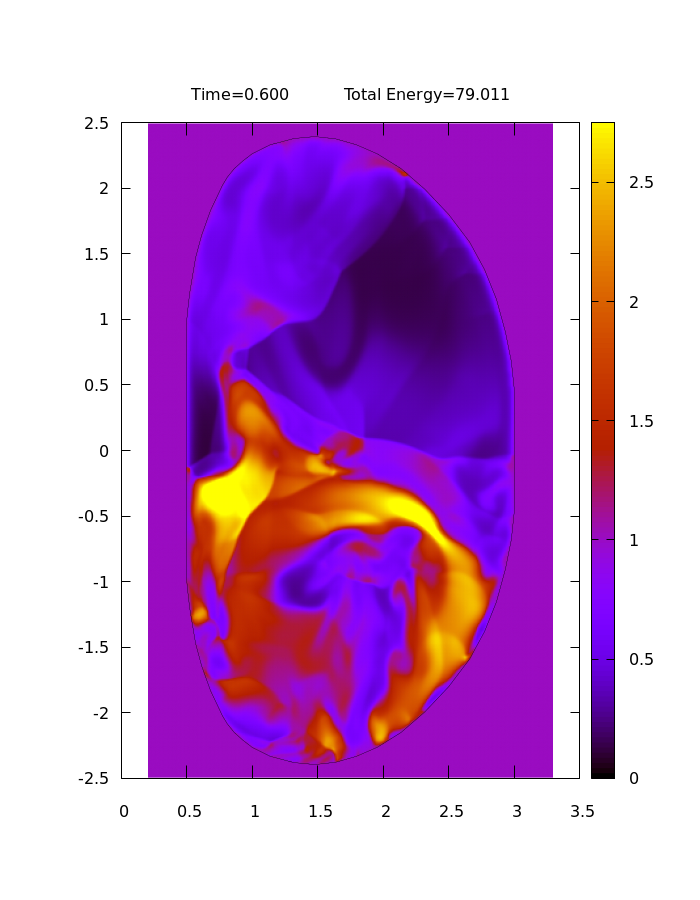
\includegraphics[width=\linewidth]{tokamak_Bz_300.png}
	\end{subfigure}
	\hspace{-5mm}
	
	\vspace{-6mm} % Negative vertical space
	
	% Row 3
	\hspace{-6mm}
	\begin{subfigure}{0.26\textwidth}
		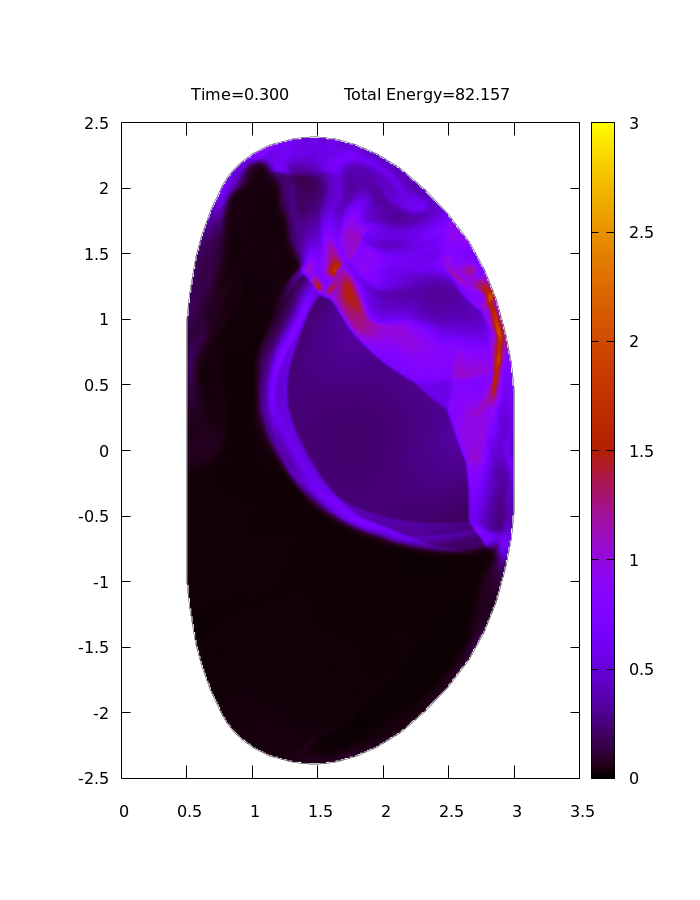
\includegraphics[width=\linewidth]{tokamak_Density_150.png}
	\end{subfigure}
	\hspace{-4mm} % Repeat negative space adjustments for each subfigure
	\begin{subfigure}{0.26\textwidth}
		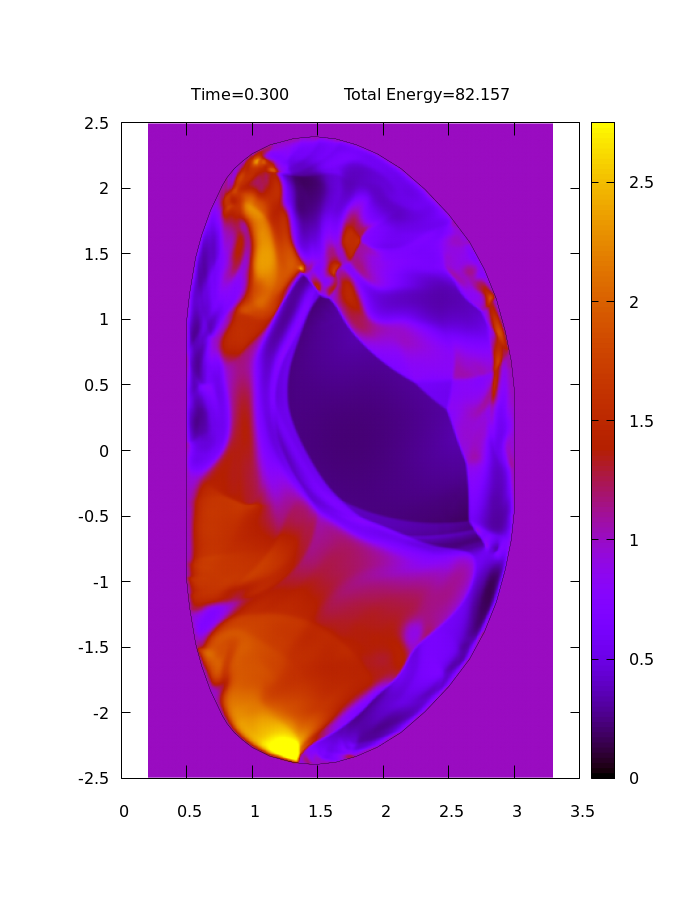
\includegraphics[width=\linewidth]{tokamak_Bz_150.png}
	\end{subfigure}
	\hspace{2mm} % Repeat negative space adjustments for each subfigure
	\begin{subfigure}{0.26\textwidth}
		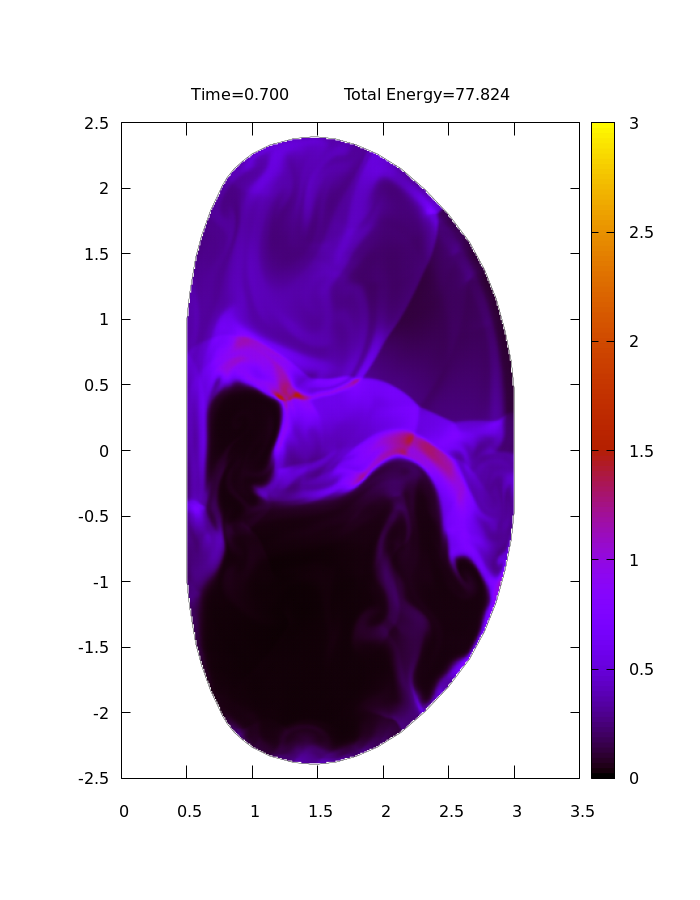
\includegraphics[width=\linewidth]{tokamak_Density_350.png}
	\end{subfigure}
	\hspace{-4mm} % Repeat negative space adjustments for each subfigure
	\begin{subfigure}{0.26\textwidth}
		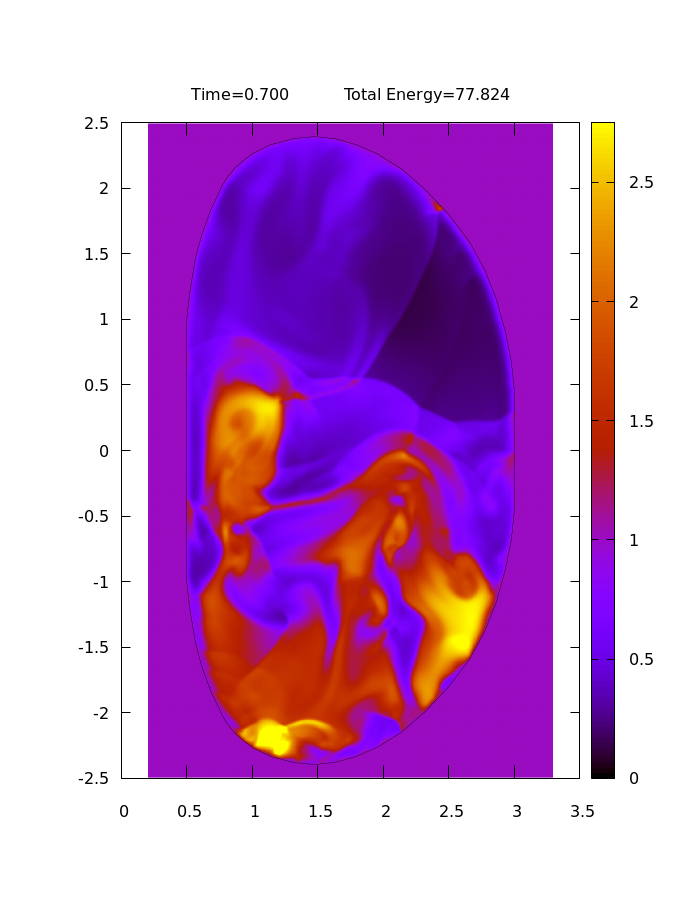
\includegraphics[width=\linewidth]{tokamak_Bz_350.png}
	\end{subfigure}
	\hspace{-6mm}
	
	\vspace{-6mm} % Negative vertical space
	
	% Row 4 
	\hspace{-6mm}
	\begin{subfigure}{0.26\textwidth}
		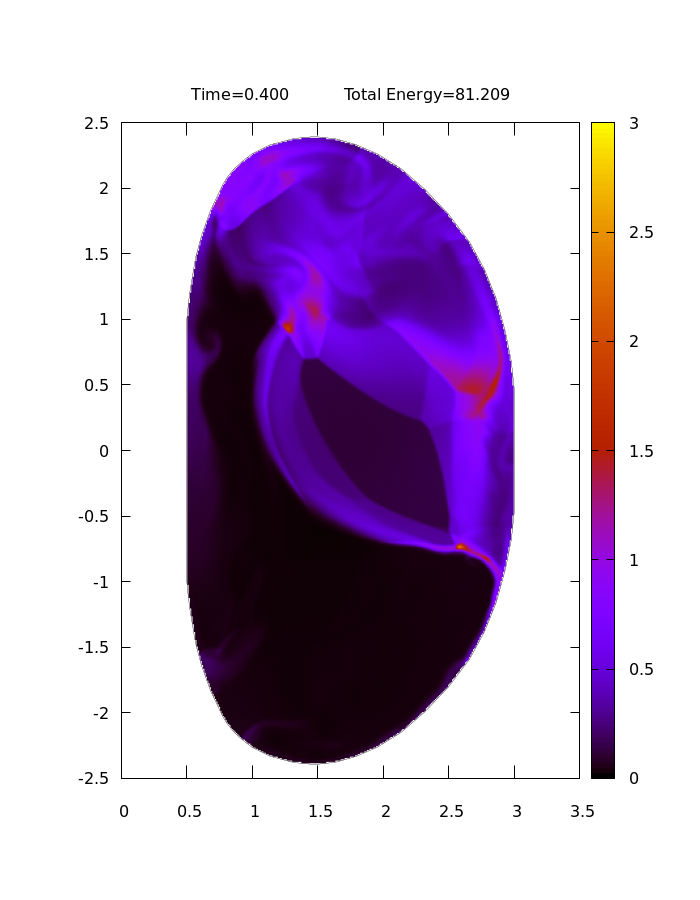
\includegraphics[width=\linewidth]{tokamak_Density_200.png}
		\caption*{Density}
	\end{subfigure}
	\hspace{-4mm} % Repeat negative space adjustments for each subfigure
	\begin{subfigure}{0.26\textwidth}
		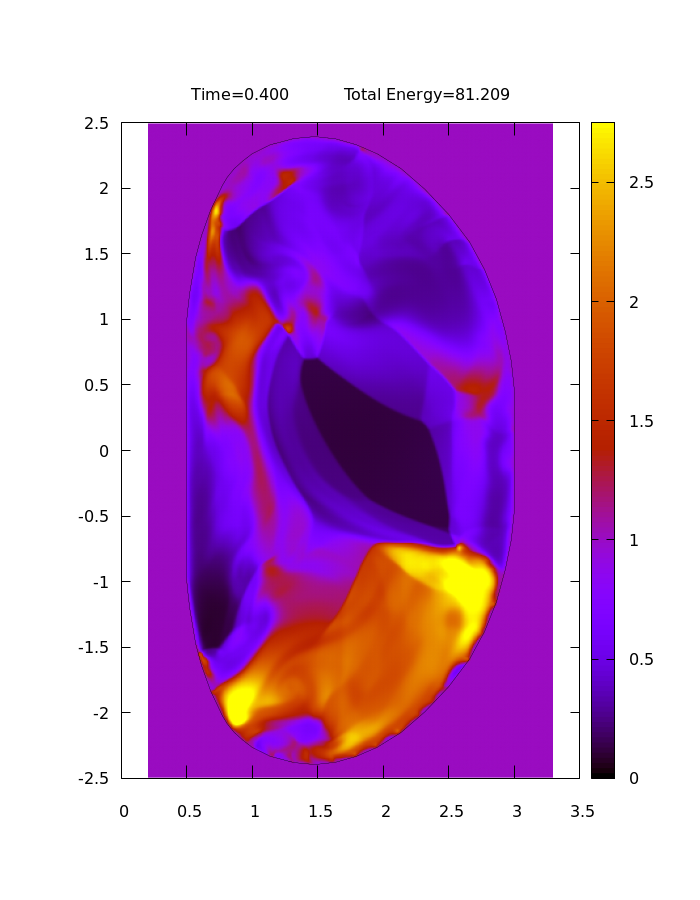
\includegraphics[width=\linewidth]{tokamak_Bz_200.png}
		\caption*{$B_z$}
	\end{subfigure}
	\hspace{2mm} % Repeat negative space adjustments for each subfigure
	\begin{subfigure}{0.26\textwidth}
		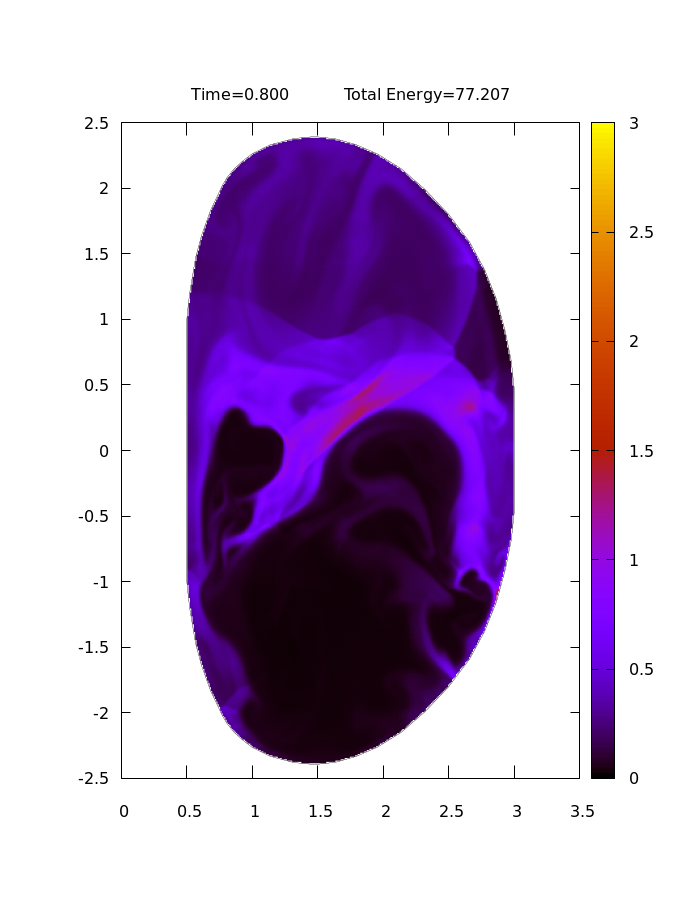
\includegraphics[width=\linewidth]{tokamak_Density_400.png}
		\caption*{Density}
	\end{subfigure}
	\hspace{-4mm} % Repeat negative space adjustments for each subfigure
	\begin{subfigure}{0.26\textwidth}
		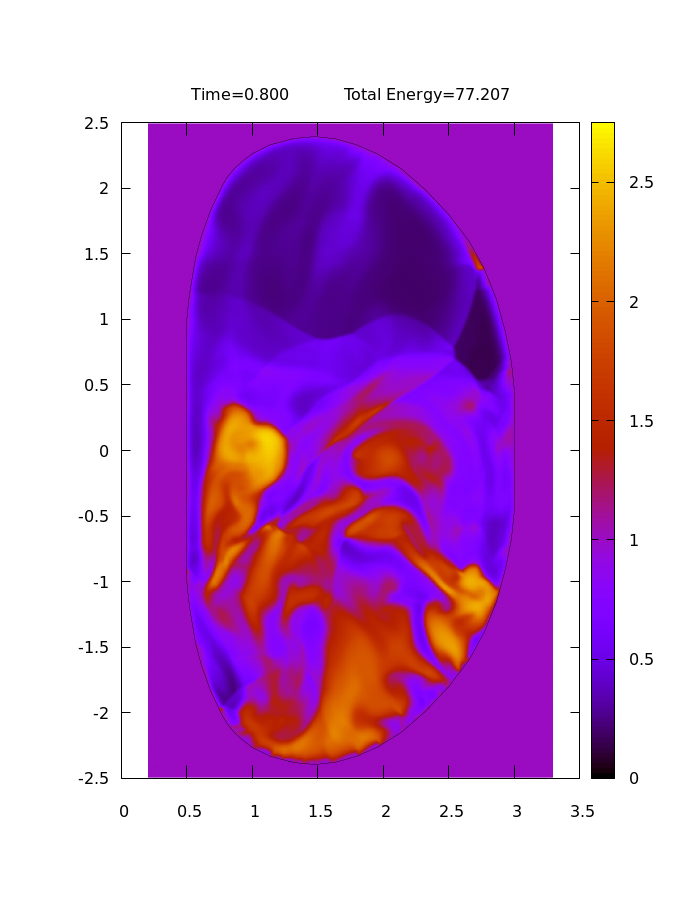
\includegraphics[width=\linewidth]{tokamak_Bz_400.png}
		\caption*{$B_z$}
	\end{subfigure}
	\hspace{-6mm}
	
	\vspace{1mm} % Negative vertical space
		
	\caption[Tokamak Application]{Simulation of cylindrical equilibrium test in a tokamak-shaped vessel. Assume the wall material is tungsten, with a resistivity of $5.6 \times 10^{-8} \, \Omega \cdot \text{m}$.}
	\label{fig:tokamak_application}
\end{figure} 


  
